\scanpage{46}
EGA IV 4º Errata et Compléments.

\deleted{$0_{\mathrm{III}}$ 10.2.1. p.18 l. -6, au lieu de ``en outre si '' lire ``si en outre''

III 4.4.12. , p.138 l.10 , au lieu de Chap V lire Chap IV 8.11.2.

III 3.4. p.119, supprimer les lignes 2 et 3, qui contiennent une promesse qui ne sera pas tenue.}
\figure{\begin{tikzpicture}\draw (0,0)..controls(.1,.2)and(.3,.35)..(.5,.5);\end{tikzpicture}}

\margin{?}
\figure{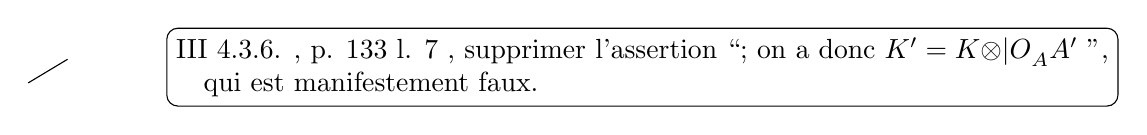
\begin{tikzpicture}[x=1cm,y=1cm]
\node[draw,rounded corners,align=left] at (0,0) {III 4.3.6. , p. 133 l. 7 , supprimer \deleted{l'assertion} ``; on a donc $K'=K\unsure{\otimes|O}_AA'$ '',\\\quad qui est manifestement faux.};
\draw (-7.8,-.2)--(-7.3,.1);
\end{tikzpicture}}

\deleted{$0_{\mathrm{IV}}$ 22.1.1. p.183 l. 12, remplacer (20.6.20) par (20.6.4) .

IV Sommaire p.223, l. 16 au lieu de ``de présentation finie'' lire ``localement de présentation finie'' ; ligne 19, après ``comme'' ajouter ``étant''.
\figure{\begin{tikzpicture}\draw (0,0)--(.65,.36);\end{tikzpicture}}

IV 3.1.10. \deleted{Ajouter à la proposition une partie (ii), où on} Supposer \inserted{d'abord} seulement $f$ quasi-compact et quasi-séparé, et \deleted{\unsure{où on}} \unsure{conclure} que $\operatorname{Ass}f_*(\underline F)\subset f(X)$, et même $\operatorname{Ass}f_*(\underline F)\subset f(\operatorname{Ass}\underline F)$ lorsque $X$ est locale ment noethérien; enfin, si de plus $f$ est entier, on a l'égalité dans cette dernière inclusion.}

\deleted{IV 3 , à la page 43, ajouter après 3.2.8. un\deleted{e}

\uline{Corollaire} 3.2.9. Soit $\underline F$ un Module cohérent sur le préschéma localement noethérien $X$. Pour toute partie \deleted{discrète} \inserted{discrète} $S$ de $X$, \inserted{i.e. loc. finie et} telle que deux points distincts de $S$ ne \unsure{soéent|soient} pas spécialisation l'un de \unsure{l'aatre|l'autre}, et \inserted{pour} tout syst tème $(\underline G(s))_{s\ S}$ de Modules quotients de \unsure{loggueur|longueur} finie de $\underline F_s$, considé-rons le Module quotient $\underline G=\underline F/\underline H$ de $\underline F$, où $\underline H$ est le noyau de l'homomorphi sme \deleted{naturel} composé $\underline F\qquad i_s(\underline F_s)\qquad i_s(\underline G(s))$, $i_s:\operatorname{Spec}k(s)\quad S$ étant le monomorphisme canonique. Alors $\underline G$ est un Module quotient cohérent de $\underline F$ sans cycles associés immergés. L'application qui, à tout système $(S,(G(s))_{s\ S})$ comme ci-dessus, associé $\underline G$, est une bijection de l'ensem ble de ces systèmes sur l'ensemble des Modules quotients cohérents de}

\mspage{45}
